\section{Control of the generalized force}\label{sec:RealizationForceVectorControl}

\begin{enumerate}
 \item Servo simulation
 \item Propeller tracking control
 \item Tricopter force filter
 \item Quadcopter force filter
 \item reconstruction of the generalized force
\end{enumerate}


The rigid body controller computes a \textit{desired} generalised force $\genForceD$ for the corresponding multicopter.
Since the force $\genForce$ itself is subject to its own actuator dynamics (see \autoref{sec:RealizationModels}), it is not possible to realize it instantaneously.
However, we can pursue to realise it reasonably fast, which is the subject of this section.
At the same time we need an accurate estimate for the current generalized force for the rigid body observer.

\subsection{Servo simulation}
The integrated servo controller uses an internal angle measurement but this is not available for the main controller.
So for validation of the servo dynamics \eqref{eq:TriModelServoDynamics} and identification of its parameters $\ServoParam[0]$ and $\ServoParam[1] $, a dedicated test bench with an incremental encoder for the tilt angle $\aServo$ was used.
Since the model is asymptotically stable a simple online simulation of the model is sufficient to get an estimate of the current servo angle.
For this a simple forward Euler discretization of \eqref{eq:TriModelServoDynamics} is implemented on the main controller
\begin{subequations}\label{eq:ServoSimulator}
\begin{align}
 \aServoObs[][k\!+\!1] &= \aServoObs[][k] + \Ts \aServoObsd[][k]
\\
 \aServoObsd[][k\!+\!1] &= \aServoObsd[][k] + \Ts( \ServoParam[0] (\aServoU[][k] - \aServoObs[][k]) - \ServoParam[1] \aServoObsd[][k])
 .
\end{align}
\end{subequations}
% \fixme{Servo param}
% \begin{align}
%  p_{\textsf{S}0} = \tfrac{K_P}{\ArmInertia}, \
%  p_{\textsf{S}1} = \tfrac{K_D}{\ArmInertia}
% \end{align}
In \autoref{fig:ServoSimRes} its result is compared to the measurement of the encoder.
To be close to the real application on the Tricopter, the propeller on the test bench is spinning with about $70\,\unit{Hz}$ during the experiment.
This explains the vibration seen in the encoder measurements.
If the propeller is switched off, the estimation error is always less than $\pm 0.5\,\unit{DEG}$.

\begin{figure}
 \centering
 \footnotesize
 \appendtographicspath{{graphics/ServoSimRes/}}
 \begingroup%
\setlength{\unitlength}{1cm}%
\begin{picture}(15.900000,10.000000)%
\put(0,0){\includegraphics{ServoSimRes.pdf}}%
\put(0.824791, 2.272028){\rotatebox{90}{\makebox(0,0)[t]{\smash{error in $\unit{RAD}$}}}}%
\put(0.648402, 6.999183){\rotatebox{90}{\makebox(0,0)[t]{\smash{$\aServo$ in $\unit{RAD}$}}}}%
\end{picture}%
\endgroup%
 \caption{Servo simulation validation}
 \label{fig:ServoSimRes}
\end{figure}

\subsection{Propeller tracking control}
The forward Euler discretization of the propeller model \eqref{eq:QuadPropDynamics} is
\begin{align}\label{eq:PropDynamics}
 \PropVel[][k\!+\!1] = \PropVel[][k] + \Ts \big( \PropParam[2] \BLDCCurr[][k] - \PropParam[3] - \PropParam[1] \big( \PropVel[][k]\big)^2 \big),
\end{align}

\paragraph*{Measurement model.}
From the commutation algorithm of the BLDC driver we get an estimate $\PropVelMeas$ of the propeller velocity which relies on its \textit{angle} $\PropAngle$ estimation used for the commutation, which is
\begin{align}
 \PropVelMeas[][k] = \tfrac{1}{\Ts} \big( \PropAngle[][k] - \PropAngle[][k\!-\!1] \big)
 .
\end{align} 
Assuming that the angular acceleration $\PropVeld$ is roughly constant within one sampling step, we have the relations
\begin{align}
 \PropAngle[][k] = \PropAngle[][k\!-\!1] + \PropVel[][k\!-\!1] \Ts + \tfrac{1}{2} \PropVeld[][k\!-\!1] \Ts^2,
\quad
 \PropVeld[][k\!-\!1] = \tfrac{1}{\Ts} \big( \PropVel[][k] - \PropVel[][k\!-\!1] \big)
 .
\end{align}
So the estimate corresponds to the mean velocity between the current and the last sampling step, \ie
\begin{align}\label{eq:PropMeaseq}
 \PropVelMeas[][k] = \tfrac{1}{2} \big( \PropVel[][k] + \PropVel[][k\!-\!1] \big)
 .
\end{align} 

\paragraph*{Observer.}
The velocity estimate $\PropVelMeas$ from the BLDC driver is quite noisy, so it should not be used directly in a feedback.
The scaled model \eqref{eq:PropDynamics} also contains the a friction parameter $\PropParam[3] = \tfrac{\BLDCFriction}{\PropInertia}$ which we like to estimate online for each propeller drive individually.
To address these two aspects, an observer for each propeller drive is implemented on the main controller.
It is essentially a copy of the discrete model \eqref{eq:PropDynamics} supplemented with a linear error feedback
\begin{subequations}\label{eq:PropObserver}
\begin{align}
 e[k] &= \PropVelMeas[][k] - \tfrac{1}{2} \big( \PropVelObs[][k] + \PropVelObs[][k-1] \big)
\\
 \PropVelObs[][k+1] &= \PropVelObs[][k] + \Ts \big( \PropParam[2] \BLDCCurr[][k] - \PropParamObs[3][k] - \PropParam[1] \big( \PropVelObs[][k]\big)^2 + \PropObsGainVel e[k] \big),
\\
 \PropParamObs[3][k+1] &= \PropParamObs[3][k] + \Ts \PropObsGainBias e[k].
\end{align}
\end{subequations}
where $\PropObsGainVel, \PropObsGainBias \in \RealNum$ are the feedback gains.
For quantitative analysis of the observer we consider the linearization of the observer error dynamics about a general expansion point $\PropVel = \PropVelStat > 0$.
Its characteristic polynomial is
\begin{align}
 \lambda^3 
 + \big( \tfrac{\Ts}{2} \big( 4 \PropParam[1] \PropVelStat + \PropObsGainVel \big) - 2 \big) \lambda^2
 + \big( 1 - \tfrac{\Ts}{2} \big( 4 \PropParam[1] \PropVelStat + \Ts \PropObsGainBias \big) \big) \lambda
 - \tfrac{\Ts}{2} \big( \PropObsGainVel + \Ts \PropObsGainBias \big)
 = 0
\end{align}
The roots $\lambda$ for the given parameters are shown in (??).

% \begin{subequations}
% \begin{align}
%  a_0 &= -\tfrac{\Ts}{2} \big( \PropObsGainVel + \Ts \PropObsGainBias \big),
% \\
%  a_1 &= 1 - \tfrac{\Ts}{2} \big( 4 \PropParam[1] \PropVelStat + \Ts \PropObsGainBias \big),
% \\
%  a_2 &= \tfrac{\Ts}{2} \big( 4 \PropParam[1] \PropVelStat + \PropObsGainVel \big) - 2,
% \\
%  a_3 &= 1.
% \end{align}
% \end{subequations}

\paragraph*{Tracking controller.}
Assume that we have a given trajectory $k \mapsto \PropVelDF[][k]$ and we want the trajectory of the propeller velocity $k \mapsto \PropVel[][k]$ (actually its estimate $\PropVelObs$) to converge to it.
Being at the sampling step $k$ the available control input is the motor current $\BLDCCurr[][k\!+\!1]$ for the \textit{next} step.
From the observer \eqref{eq:PropObserver} we have estimates for the velocity $\PropVelObs[][k\!+\!1]$ and the friction $\PropParamObs[3][k\!+\!1]$ at the next sampling step.
Taking this into account we propose the control law:
\begin{subequations}\label{PropCtrlLaw}
\begin{align}
 e[k\!+\!1] &= \PropVelDF[][k\!+\!1] - \PropVelObs[][k\!+\!1],
\\
 \BLDCCurr[][k\!+\!1] &= \tfrac{1}{\PropParam[2]} \big( \tfrac{\PropVelDF[][k+2] - \PropVelDF[][k+1]}{\Ts} + \PropParam[1] \big( \PropVelDF[][k\!+\!1] \big)^2 + \PropParamObs[3][k\!+\!1] + \PropCtrlGain e[k\!+\!1] \big),
\end{align}
\end{subequations}
It is essentially a (shifted) copy of the discrete model \eqref{eq:PropDynamics} supplemented with a linear error feedback with the gain $\PropCtrlGain \in \RealNum$.
Plugging the control law \eqref{PropCtrlLaw} into the model \eqref{eq:PropDynamics} and assuming the observer has converged, \ie $\PropVelObs[][k] = \PropVel[][k]$ and $\PropParamObs[3][k] = \PropParam[3]$, yields the tracking error dynamics
\begin{align}
 e[k\!+\!1] + \big( \Ts (2 \PropParam[1] \PropVel[][k] + \PropCtrlGain) - 1 \big) e[k] + \Ts \PropParam[1] \big( e[k] \big)^2 = 0.
\end{align}
For a the linearization about the expansion point $e = 0$, $\PropVel = \PropVelStat$ the corresponding characteristic polynomial has the root
\begin{align}
 \lambda = 1 - \Ts (2 \PropParam[1] \PropVelStat + \PropCtrlGain).
\end{align}


\begin{figure}
 \centering
 \footnotesize
 \appendtographicspath{{graphics/PropCtrlRes/}}
 \begingroup%
\setlength{\unitlength}{1cm}%
\begin{picture}(15.900000,17.000000)%
\put(0,0){\includegraphics{PropCtrlRes.pdf}}%
\put(0.980045, 8.981390){\rotatebox{90}{\makebox(0,0)[t]{\smash{error in $\unit{N}$}}}}%
\put(1.372021, 13.880619){\rotatebox{90}{\makebox(0,0)[t]{\smash{$\PropForce$ in $\unit{N}$}}}}%
\put(8.830640, 0.302626){\makebox(0,0)[b]{\smash{$t$ in $\unit{s}$}}}%
\put(0.744859, 2.363751){\rotatebox{90}{\makebox(0,0)[t]{\smash{$\hat{\tau}_{\mathsf{MB}}$ in $\unit{Nm}$}}}}%
\put(1.195632, 5.665956){\rotatebox{90}{\makebox(0,0)[t]{\smash{$\BLDCCurr$ in $\unit{A}$}}}}%
\end{picture}%
\endgroup%
 \caption{Propeller control validation}
 \label{fig:PropCtrlRes}
\end{figure}

\subsection{Tricopter force control}
The generalized force $\genForce$ on the \Tricopter is a static transformation of the propeller velocities $\PropVel[1], \ldots \PropVel[3]$ and the servo angles $\aServo[1],\ldots,\aServo[3]$ as given in \eqref{eq:TriActuatorTrafo}.
For a given desired generalized force $\genForceD$ we can (partially) invert this relation to obtain the corresponding propeller thrusts $\PropForceD[1], \ldots \PropForceD[3]$ and servo angles $\aServoD[1],\ldots,\aServoD[3]$ as
\begin{align}\label{eq:TriInvActuatorTrafo}
 \F_{\idxDes}^\mathsf{VH} = B^{-1} \genForceD,
\quad
 \PropForceD[j] = \sqrt{(\F_{\idxDes j}^\mathsf{V})^2 + (\F_{\idxDes j}^\mathsf{H})^2},
\quad
 \aServoD[j] = \atanTwo(\F_{\idxDes j}^\mathsf{H}, \F_{\idxDes j}^\mathsf{V}),
\quad j = 1,2,3.
\end{align}
In addition the computed values are saturated to $0.3\,\unit{N} \leq \PropForceD[i] \leq 7.0\,\unit{N}$ and $-45^\circ\leq \aServoD[i] \leq 45^\circ, i=1,2,3$ to incorporate the practical limitations of the actuators.
The desired servo angles $\aServoD[i]$ are directly forwarded to the servo controllers.
In contrast, for the desired thrusts $\PropForce[i]$ a first order filter is applied:
\begin{align}\label{eq:PropPrefilter}
 \PropForceDF[][k\!+\!2] = \lambda_{\mathsf{Filt}} \PropForceDF[][k\!+\!1] + (1-\lambda_{\mathsf{Filt}}) \PropForceD[][k\!+\!1],
\qquad
 \PropVelDF[][k\!+\!2] = \sqrt{\sfrac{\PropForceDF[][k\!+\!2]}{\kappaF}}.
\end{align}
This yields the desired propeller velocities $\PropVelDF[i][k+1]$ and $\PropVelDF[i][k+2]$ for the next \textit{two} sampling steps which are required for the propeller \textit{tracking} controller.
After the propeller controller has converged, \ie $\PropForce[i] = \PropForceDF[i]$, the thrust dynamic is completely determined by this filter.

Overall we can combine the discrete servo dynamics \eqref{eq:ServoSimulator}, the thrust filter \eqref{eq:PropPrefilter} and the static transformations \eqref{eq:TriActuatorTrafo} and \eqref{eq:TriInvActuatorTrafo} to obtain a nonlinear dynamic system with the input $\genForceD$ and the output $\genForce$, the \textit{\Tricopter actuator dynamics}.
For a quantitative analysis its first order approximation about a general expansion point $(\PropForceStat[1], \PropForceStat[2], \PropForceStat[3], \aServoStat[1], \aServoStat[2], \aServoStat[3])$ is considered.
Using the $z$-transformation $\ZTrafo{\cdot}$ the linearized dynamics between $\genForce$ and $\genForceD$ can be written as 
\begin{align}
 \ZTrafo{\Delta \genForce} = \GenForceTransferFunction(z) \, \ZTrafo{\Delta \genForceD}.
\end{align}
The discrete transfer function
\begin{align}\label{eq:TriActuatorTransferFunction}
 \GenForceTransferFunction(z) = J \diag(\ThrustTransferFunction(z), \ThrustTransferFunction(z), \ThrustTransferFunction(z), \ServoTransferFunction(z), \ServoTransferFunction(z), \ServoTransferFunction(z)) J^{-1}
\end{align}
consists of $\ThrustTransferFunction(z)$, the transfer function of the thrust filter \eqref{eq:PropPrefilter}, $\ServoTransferFunction(z)$, the transfer function of the controlled servo \eqref{eq:ServoSimulator}:
\begin{align}
 \ThrustTransferFunction(z) = \frac{1-c_F}{z-c_F},
\qquad
 \ServoTransferFunction(z) = \frac{\ServoParam[0] \Ts^2}{(z-1)^2 + \ServoParam[1]\Ts (z-1) + \ServoParam[0] \Ts^2}
 .
\end{align}
and $J$ is the Jacobian matrix of the force transformation \eqref{eq:TriActuatorTrafo} at the expansion point.
\begin{align}
 %\underbrace{\begin{bmatrix} \Delta \Fx \\ \Delta \Fy \\ \Delta \Fz \\ \Delta \taux \\ \Delta \tauy \\ \Delta \tauz \end{bmatrix}}_{\Delta \genForce}
 J = B
 \begin{bmatrix}
  \cos\aServoStat[1] & 0 & 0 & -\PropForceStat[1] \sin\aServoStat[1] & 0 & 0 \\
  0 & \cos\aServoStat[2] & 0 & 0 & -\PropForceStat[2] \sin\aServoStat[2] & 0 \\
  0 & 0 & \cos\aServoStat[3] & 0 & 0 & -\PropForceStat[3] \sin\aServoStat[3] \\
  \sin\aServoStat[1] & 0 & 0 & \PropForceStat[1] \cos\aServoStat[1] & 0 & 0 \\
  0 & \sin\aServoStat[2] & 0 & 0 & \PropForceStat[2] \cos\aServoStat[2] & 0 \\
  0 & 0 & \sin\aServoStat[3] & 0 & 0 & \PropForceStat[3] \cos\aServoStat[3] \\
 \end{bmatrix}
% \begin{bmatrix} \Delta \PropForce[1] \\ \Delta \PropForce[2] \\ \Delta \PropForce[3] \\ \Delta \aServo[1] \\ \Delta \aServo[2] \\ \Delta \aServo[3] \end{bmatrix}
 .
\end{align}
Note that $\PropForceStat$ cancels out in \eqref{eq:TriActuatorTransferFunction}, \ie $\GenForceTransferFunction$ is independent of it.

From the structure of $\GenForceTransferFunction$ in \eqref{eq:TriActuatorTransferFunction} it is clear that its entries are linear combinations of the transfer functions the the thrust and the servos, $\ThrustTransferFunction$ and $\ServoTransferFunction$.
Also it is evident that if $\ThrustTransferFunction = \ServoTransferFunction$, then $\GenForceTransferFunction$ would be diagonal.
Since this is not the case we do have off-diagonal entries in the transfer matrix $\GenForceTransferFunction$.
This so-called crosstalk between the components of the generalized force $\genForce$ depends mainly on the expansion point of the servo angles $\aServoStat$.

For a better quantitative analysis of the off-diagonal entries of $\GenForceTransferFunction$, the transfer function is normalized as $\GenForceTransferFunctionNorm = S^{-1} \GenForceTransferFunction S $ where $S = \diag(F_{\mathsf{x,Max}}, \ldots, \tau_{\mathsf{z,Max}})$ contains the maximal magnitudes of the corresponding forces and torques.
\autoref{fig:BodeTriActorDyn} shows exemplary the bode magnitude plot of $\GenForceTransferFunctionNorm$ for the hover case $\aServoStat = [0,0,0]^\top$ (left) and for a forward force with $\aServoStat = [\sfrac{\pi}{4},0,-\sfrac{\pi}{4}]^\top$ (right).
In the hover case the diagonal entries for $\Fz$, $\taux$ and $\tauy$ coincide with the thrust dynamics $\ThrustTransferFunction$, whereas the diagonal entries for $\Fx$ and $\Fy$ coincide with the servo dynamics $\ServoTransferFunction$.
The diagonal entry for $\tauz$ is dominated by the servo dynamics $\ServoTransferFunction$ but also has a small influence from $\ThrustTransferFunction$ due to the propeller drag (terms involving $\kappaT$ in \eqref{eq:TriActuatorTrafo}).
The propeller drag is also responsible for the small off-diagonal entries in the hover case.
For the forward force case it is evident that the diagonal entries are linear combinations of $\ThrustTransferFunction$ and $\ServoTransferFunction$.
Furthermore, the off-diagonal entries have a significantly larger magnitude.

\begin{figure}
 \centering
 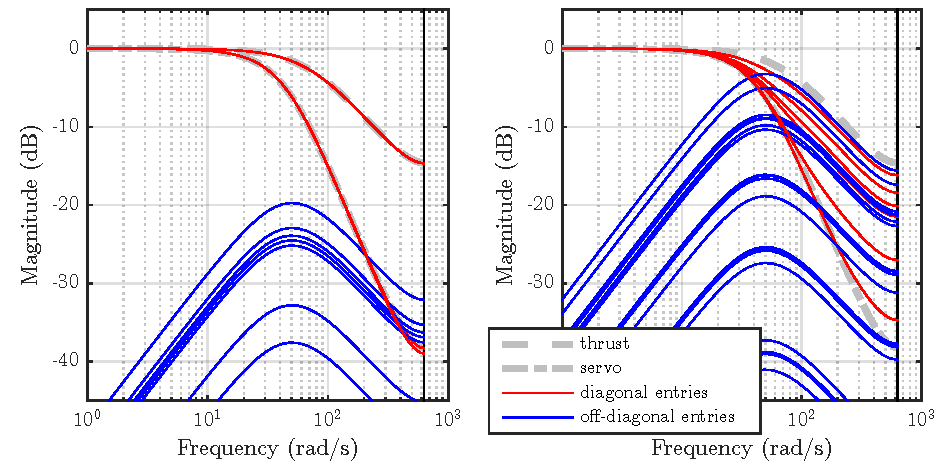
\includegraphics{graphics/TriActuatorDynamics/BodeTriActorDyn.pdf}
 \caption{Bode magnitude plot of the normalized \Tricopter actuator dynamics transfer function $\GenForceTransferFunctionNorm$ at different expansion points}
 \label{fig:BodeTriActorDyn}
\end{figure}


% \begin{figure}[htb]
%  \centering
%  \input{graphics/PropCtrlBlock.pdf_tex}
%  \caption{Structure of the Propeller control algorithm}
%  \label{fig:PropCtrlBlock}
% \end{figure}


\subsection{Quadcopter force vector control}
\paragraph{Model.}
The model of the generalized force on the quadcopter from \eqref{eq:QuadActuatorTrafo} can be split into a static part $\genForceQuadStat$, proportional to the squares of the propeller velocities $\PropVel$, and a dynamic part $\genForceQuadDyn$ proportional to the propeller accelerations $\PropVeld$, as
\begin{align}\label{eq:QuadForceVelctorModel}
% \underbrace{\begin{bmatrix} \Fz \\ \taux \\ \tauy \\ \tauz \end{bmatrix}}_{\genForceQuad}
 \genForceQuad(\PropVel, \PropVeld)
 =
 \underbrace{
 \overbrace{\begin{bmatrix}
  \kappaF & \kappaF & \kappaF & \kappaF \\
  0 & \kappaF\ArmRadius & 0 & -\kappaF\ArmRadius \\
  -\kappaF\ArmRadius & 0 & \kappaF\ArmRadius & 0 \\
  -\kappaT & \kappaT & -\kappaT & \kappaT \\
 \end{bmatrix}}^{B}
 %\underbrace{
 \begin{bmatrix} \PropVel[1]^2 \\ \PropVel[2]^2 \\ \PropVel[3]^2 \\ \PropVel[4]^2 \end{bmatrix}
 %}_{\PropForce[]}
 }_{\genForceQuadStat(\PropVel)}
 -
 \underbrace{\begin{bmatrix} 0 \\ 0 \\ 0 \\ \JP (\PropVeld[1] - \PropVeld[2] + \PropVeld[3] - \PropVeld[4]) \end{bmatrix}}_{\genForceQuadDyn(\PropVeld)}
 .
\end{align}

\paragraph{Filter dynamics.}
The task here is to design a filter which outputs the desired propeller velocities $\PropVel[][k]$ and $\PropVel[][k+1]$ for the next two sampling steps based on the given desired generalized force $\genForceQuadD[k]$.
Note that $\genForceQuad$ is \textit{not} a flat output of \eqref{eq:QuadForceVelctorModel}, so a simple low-pass filter for $\genForceQuadD$ does not do the trick.
However, the propeller velocities $\PropVel$ form a flat output and so we propose the following continuous time filter
\begin{align}\label{eq:QuadActuatorFilterDesign}
 \tfrac{\d^2}{\d t^2} \big(\genForceQuadStat(\PropVelDF)\big) + K_1 \tfrac{\d}{\d t} \big(\genForceQuadStat(\PropVelDF)\big) + K_0 \big( \genForceQuad(\PropVelDF,\PropVelDFd) - \genForceQuadD \big) = 0
 .
\end{align}
With introduction of the auxiliary state $\hat{h} = \tfrac{\d}{\d t} \big(\genForceQuadStat(\PropVelDF)\big) + K_1 \genForceQuadStat(\PropVelDF)$ this can be rewritten in an explicit first order form
\begin{subequations}\label{eq:QuadcopterActuatorFilter}
\begin{align}
 \PropVelDFd &= \diag(2 \kappaF \PropVelDF)^{-1} B^{-1} \big( \hat{h} - K_1 \genForceQuadStat(\PropVelDF) \big),
\\
 \dot{\hat{h}} &= K_0 \big( \genForceQuadD - \genForceQuad(\PropVelDF,\PropVelDFd) \big).
\end{align}
\end{subequations}
For the time discrete implementation we add the forward Euler approximation of the derivatives
\begin{align}\label{eq:QuadcopterActuatorFilterDiscretization}
 \PropVelDF[][k\!+\!1] = \PropVelDF[][k] + \Ts \PropVelDFd[][k],
\qquad
 \hat{h}[k\!+\!1] = \hat{h}[k] + \Ts \dot{\hat{h}}[k].
\end{align}
With this representation of the filter dynamics it is very simple to add a saturation $\PropVelMin \leq \PropVelDF \leq \PropVelMax$ to take into account the practical limitations of the propellers.
The combination of \eqref{eq:QuadcopterActuatorFilter} and \eqref{eq:QuadcopterActuatorFilterDiscretization} constitute a time discrete nonlinear system with the input $\genForceQuadD[k]$ and the output $\PropVelDF[][k]$, $\PropVelDF[][k+1]$, the \textit{quadcopter actuator dynamics}.  

\paragraph{Tuning.}
The filter gains $K_1$ and $K_2$ are chosen as diagonal matrices and for symmetry considerations the gains corresponding to $\taux$ and $\tauy$ are identical, \ie
\begin{align}
 K_0 = \diag(\kPMag, \kPTilt, \kPTilt, \kPHead),
\qquad
 K_1 = \diag(\kDMag, \kDTilt, \kDTilt, \kDHead).
\end{align}
For a quantitative analysis of the actuator dynamics we consider its linearization for a general expansion point $(\PropVelStat[1], \ldots, \PropVelStat[4]) \in [\PropVelMin, \PropVelMax]^4$.
Using the $z$-transformation we get the following transfer matrix 
\begin{align}
 \ZTrafo{\Delta \genForce} = \GenForceTransferFunction(z) \, \ZTrafo{\Delta \genForceD},
\qquad
 \GenForceTransferFunction(z) =
 \begin{bmatrix}
  G_{11}(z) & 0 & 0 & 0 \\
  0 & G_{22}(z) & 0 & 0 \\
  0 & 0 & G_{33}(z) & 0 \\
  G_{41}(z) & G_{42}(z) & G_{43}(z) & G_{44}(z) \\
 \end{bmatrix}
\end{align}
with the components
\begin{subequations}\label{eq:QuadActuatorDynTransferComponents}
\begin{align}
% G_{11}(z) &= \frac{\kPMag\Ts^2}{(z-1)^2 + \kDMag\Ts (z-1) + \kPMag\Ts^2}
 G_{11}(z) &= \frac{\kPMag}{\big(\tfrac{z-1}{\Ts}\big)^2 + \kDMag \tfrac{z-1}{\Ts} + \kPMag}
\\
 G_{22}(z) = G_{33}(z) &= \frac{\kPTilt}{\big(\tfrac{z-1}{\Ts}\big)^2 + \kDTilt \tfrac{z-1}{\Ts} + \kPTilt}
\\
 G_{44}(z) &= \frac{\kPHead(p_4\tfrac{z-1}{\Ts} + 1)}{\big(\tfrac{z-1}{\Ts}\big)^2 + (\kPHead p_4 + \kDTilt) \tfrac{z-1}{\Ts} + \kPHead}
\\
 G_{4j}(z) &= \frac{p_j\,G_{jj}(z)\,\big(\tfrac{z-1}{\Ts}\big)^2 (\tfrac{z-1}{\Ts} + \kDHead)}{\big(\tfrac{z-1}{\Ts}\big)^2 + (\kPHead p_4 + \kDTilt) \tfrac{z-1}{\Ts} + \kPHead}, \quad j=1,2,3
\end{align}
\end{subequations}
and the (expansion point dependent) model parameters
\begin{subequations}
\begin{align}
 p_1 &= \tfrac{\PropInertia}{8\kappaF} \left( \tfrac{1}{\PropVelStat[4]} - \tfrac{1}{\PropVelStat[3]} + \tfrac{1}{\PropVelStat[2]} - \tfrac{1}{\PropVelStat[1]} \right),&
 p_2 &= \tfrac{\PropInertia}{4\kappaF\ArmRadius} \left( \tfrac{1}{\PropVelStat[2]} - \tfrac{1}{\PropVelStat[4]} \right),
\\
 p_4 &= \tfrac{\PropInertia}{8\kappaT} \left( \tfrac{1}{\PropVelStat[1]} + \tfrac{1}{\PropVelStat[2]} + \tfrac{1}{\PropVelStat[3]} + \tfrac{1}{\PropVelStat[4]} \right),&
 p_3 &= \tfrac{\PropInertia}{4\kappaF\ArmRadius} \left( \tfrac{1}{\PropVelStat[1]} - \tfrac{1}{\PropVelStat[3]} \right).
\end{align}
\end{subequations}
The transfer behaviors for $\Fz$, $\taux$ and $\tauy$ are uncorrelated and independent of the expansion point.
Their parameters are chosen to form a second order Butterworth filter.

Unfortunately, the transfer behavior for $\tauz$ is not that nice:
It is in general affected by all components of $\genForceD$ and the corresponding transfer functions $G_{4j}, j=1,\ldots,4$ depend on the expansion point.
However, for the hover case $\PropVelStat[1] = \PropVelStat[2] = \PropVelStat[3] = \PropVelStat[4] = \sqrt{\sfrac{m \gravityAccConst}{4\kappaF}}$ we have $p_1=p_2=p_3=0$ and $p_4 = \tfrac{\PropInertia}{\kappaT}\sqrt{\sfrac{\kappaF}{m \gravityAccConst}}$.
We choose $\kDHead = \sfrac{1}{p_4} = \tfrac{\kappaT}{\PropInertia}\sqrt{\sfrac{m \gravityAccConst}{\kappaF}}$ such that \textit{at this particular expansion point} we have a pole-zero cancellation.
The remaining parameter $\kPHead$ is then used to adjust the cut-off frequency of the filter.

\autoref{fig:BodeQuadActorDyn} shows the Bode magnitude plot of the normalized transfer matrix $\GenForceTransferFunctionNorm$ coefficients from \eqref{eq:QuadActuatorDynTransferComponents} with the used filter parameters.
The left side corresponds to the most common hover case $\PropVelStat[1] = \PropVelStat[2] = \PropVelStat[3] = \PropVelStat[4] = \sqrt{\sfrac{m \gravityAccConst}{4\kappaF}}$ whereas the right side captures the ``worst case`` expansion points where $(\PropVelStat[1], \ldots,\PropVelStat[4]) \in \{ \PropVelMin, \PropVelMax\}^4$.
Obviously the pole-zero cancellation only holds for the hover case but even for the worst case points $G_{44}$ only differs slightly from its design.
Furthermore one can see that the influence of the off-diagonal entries is restricted to high frequencies.

\begin{figure}[ht]
 \centering
 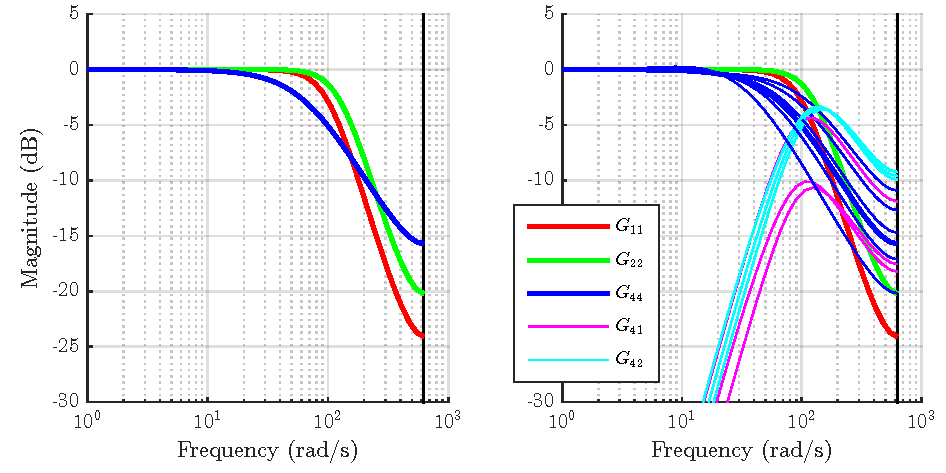
\includegraphics{graphics/QuadActuatorDynamics/BodeQuadActorDyn.pdf}
 \caption{Bode magnitude plot of the normalized transfer matrix $\GenForceTransferFunctionNorm$ at different expansion points}
 \label{fig:BodeQuadActorDyn}
\end{figure}

\paragraph{Comparison to static approach.}
The proposed filter \eqref{eq:QuadActuatorFilterDesign} might seem complicated.
In particular one might argue that the dynamic part $\genForceQuadDyn$ in the model \eqref{eq:QuadForceVelctorModel} is neglectable, as is done in most publications on this subject.

To answer this question we can replace \eqref{eq:QuadActuatorFilterDesign} by
\begin{align}\label{eq:QuadActuatorFilterDesignTraditional}
 \tfrac{\d^2}{\d t^2} \big(\genForceQuadStat(\PropVelDF)\big) + K_1 \tfrac{\d}{\d t} \big(\genForceQuadStat(\PropVelDF)\big) + K_0 \big( \genForceQuadStat(\PropVelDF) - \genForceQuadD \big) = 0
\end{align}
what essentially neglects the dynamics part $\genForceQuadDyn$ in the generalized force $\genForceQuad = \genForceQuadStat + \genForceQuadDyn$.
As before we now consider the transfer matrix $\GenForceTransferFunction$ for the linearized filter at a general expansion point.
The components differing from \eqref{eq:QuadActuatorDynTransferComponents} are
\begin{align}\label{eq:QuadActuatorDynTransferTraditionalComponents}
 G_{44}(z) = \frac{\kPHead(p_4\tfrac{z-1}{\Ts} + 1)}{\big(\tfrac{z-1}{\Ts}\big)^2 + \kDTilt \tfrac{z-1}{\Ts} + \kPHead}
\qquad
 G_{4j}(z) = p_j\,\tfrac{z-1}{\Ts}\,G_{jj}(z), \ j=1,2,3.
\end{align}
Now one can chose the gains $K_0$ and $K_1$ such that \eqref{eq:QuadActuatorFilterDesignTraditional} forms 4 decoupled second order Butterworth filters with inputs $\genForceQuadD$ and outputs $\genForceQuadStat$.
However, since the real force on the quadcopter does contain the dynamic part as well the behavior from $\genForceQuadD$ to $\genForceQuad = \genForceQuadStat + \genForceQuadDyn$ is quite different, as can be seen in \eqref{eq:QuadActuatorDynTransferTraditionalComponents}.
The Bode magnitude plot of the transfer functions is displayed in \autoref{fig:BodeQuadActorDynTraditional} on the left side.
Even for the hover case (thick lines) the transfer function $G_{44}$ for $\tauz$ has an unacceptable overshot.

In oder to improve the behavior we can do the same as before: adjust the parameters in $G_{44}$, \ie $\kPHead$ and $\kDHead$, such that there is a pole-zero cancelation at the hover expansion point.
The resulting Bode magnitude plot is shown on the right side of \autoref{fig:BodeQuadActorDynTraditional}.
It is already a significant improvement compared to the right side but is much worse as the previous result shown in \autoref{fig:BodeQuadActorDyn}.
Moreover, the magnitude of the off-diagonal transfer functions at low frequencies is much higher for both cases in \autoref{fig:BodeQuadActorDynTraditional} than in \autoref{fig:BodeQuadActorDyn}.

\begin{figure}[ht]
 \centering
 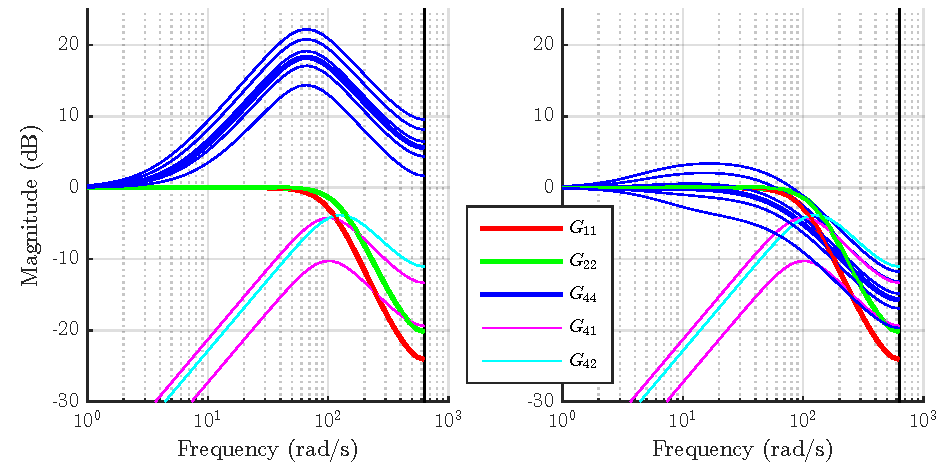
\includegraphics{graphics/QuadActuatorDynamics/BodeQuadActorDynTraditional.pdf}
 \caption{Bode magnitude plot of the normalized transfer matrix $\GenForceTransferFunctionNorm$ at different expansion points (static approach)}
 \label{fig:BodeQuadActorDynTraditional}
\end{figure}

Overall this discussion should justify the filter design in \eqref{eq:QuadActuatorFilterDesign} and justify the consideration of the dynamic model \eqref{eq:QuadForceVelctorModel} for the present case.
For other quadcopters with smaller ratios $\sfrac{\PropInertia}{\kappaT}$ or less aggressively tuned multicopters like the previously discussed tricopter, however, the situation can be different.


% \subsection{Propeller aerodynamics}
% picture of the propeller, its geometric center and the forces
% 
% The main purpose of a propeller is to generate a force $\vect{F} = \PropForce \,\vect{b}_3$ in its spinning direction $\vect{b}_3$, but the actual aerodynamics contain several mode effects.
% 
% \paragraph{Aerodynamic model.}
% In the following we discuss the propeller model proposed in \cite{Martin:AccelerometerFeedback}.
% They claim that it is based on general blade element theory from \cite{Johnson:HelicopterTheory}, but is adopted to the specific conditions of their quadcopter which is about the same size as the one build for this work. 
% The proposed model is\footnote{There is probably a typo in \cite{Martin:AccelerometerFeedback}, eq.\ (2), the definition is corrected such that their result in eq.\ (7) is plausible.}
% \begin{subequations}\label{eq:PropellerForceTorque}
% \begin{alignat}{10}
% %  \vect{F} & \ = \ &
% %  \kappa_F &\PropVel^2 \vect{b}_3&
% %  \ &- \ &
% %  &\PropVel ( \lambda_1 \vect{v}^\bot + \lambda_2 \vect{\omega} \times \vect{b}_3 )&
% %  \ &- \ &
% %  \PropDir &\PropVel (\lambda_3 \vect{v} \times \vect{b}_3 + \lambda_4 \vect{\omega}^\bot)
% % \\
% %  \vect{\tau} & \ = \ &
% %  -\kappa_\tau \PropDir &\PropVel^2 \vect{b}_3&
% %  \ &- \ &
% %  \PropDir &\PropVel ( \mu_1 \vect{v}^\bot - \mu_2 \vect{\omega} \times  \vect{b}_3 )&
% %  \ &+ \ &
% %  &\PropVel (\mu_3 \vect{v} \times \vect{b}_3 - \mu_4 \vect{\omega}^\bot)
%  \vect{F} & \ = \ &
%  \kappa_F &\PropVel^2 \vect{b}_3&
%  \ &+ \ &
%  \big( \phantom{\PropDir} &( \lambda_1 \vect{v} \times \vect{b}_3 + \lambda_2 \vect{\omega} )&
%  \ &+ \ &
%  \PropDir &(\lambda_3 \vect{v} + \lambda_4 \vect{\omega} \times \vect{b}_3) \big) \times (\PropVel \vect{b}_3)
% \\
%  \vect{\tau} & \ = \ &
%  -\kappa_\tau \PropDir &\PropVel^2 \vect{b}_3&
%  \ &+ \ &
%  \big( \PropDir &( \mu_1 \vect{v} \times \vect{b}_3 - \mu_2 \vect{\omega} )&
%  \ &- \ &
%  &(\mu_3 \vect{v} - \mu_4 \vect{\omega} \times \vect{b}_3) \big) \times (\PropVel \vect{b}_3)
% \end{alignat}
% \end{subequations}
% where $\PropVel > 0$ is the angular velocity of the propeller and $\PropDir = 1$ ($\PropDir = -1$) for a counterclockwise (clockwise) rotating propeller.
% The vectors $\vect{v}$ and $\vect{\omega}$ are the velocity with which the geometric center of the propeller moves in the surrounding space.
% %The accent $\vect{a}^\bot = \vect{b}_3 \times (\vect{a} \times \vect{b}_3) = \vect{a} - \sProd{\vect{a}}{\vect{b}_3}\vect{b}_3$ indicates a projection of a vector in the propeller plane.
% The model \eqref{eq:PropellerForceTorque} introduces 10 positive parameters $\kappa_F$, $\kappa_\tau$, $\lambda_1,\ldots,\lambda_4$ and $\mu_1,\ldots,\mu_4$ that depend the propeller geometry.
% 
% \paragraph*{Resulting generalized force.}
% Let $P_i$ be the body index of the $i$-th propeller, than we can write \eqref{eq:PropellerForceTorque} as
% \begin{align}
%  \underbrace{\begin{bmatrix}[1.1] \bodyForce{0}{P_i}{1} \\ \bodyForce{0}{P_i}{2} \\ \bodyForce{0}{P_i}{3} \\ \bodyTorque{0}{P_i}{1} \\ \bodyTorque{0}{P_i}{1} \\ \bodyTorque{0}{P_i}{2} \\ \bodyTorque{0}{P_i}{3} \end{bmatrix}}_{\bodyGenForce{0}{P_i}{}}
%  &=
%  \PropVel[i]^2 \underbrace{\begin{bmatrix}[1.2] 0 \\ 0 \\ \kappa_F \\ 0 \\ 0 \\ -\PropDir[i] \kappa_\tau \end{bmatrix}}_{\kappa_{i}}
%  + \, \PropVel[i]
%  \underbrace{\begin{bmatrix}[1.2]
%   -\lambda_1 & \PropDir[i] \lambda_3 & 0  & -\PropDir[i] \lambda_4 & \lambda_2 & 0 \\
%   -\PropDir[i] \lambda_3 & -\lambda_1 & 0 & -\lambda_2 & -\PropDir[i] \lambda_4 & 0 \\
%   0 & 0 & 0 & 0 & 0 & 0 \\
%   -\PropDir[i]\mu_1 & \mu_3 & 0 & -\mu_4 & -\PropDir[i] \mu_2 & 0 \\
%   \mu_3 & -\PropDir[i] \mu_1 & 0 & \PropDir[i]\mu_2 & -\mu_4 & 0 \\
%   0 & 0 & 0 & 0 & 0 & 0
%  \end{bmatrix}}_{K_{i}}
%  \underbrace{\begin{bmatrix}[1.2] \bodyLinVel{0}{P_i}{1} \\ \bodyLinVel{0}{P_i}{2} \\ \bodyLinVel{0}{P_i}{3} \\ \bodyAngVel{0}{P_i}{1} \\ \bodyAngVel{0}{P_i}{2} \\ \bodyAngVel{0}{P_i}{3} \end{bmatrix}}_{\bodyVel{0}{P_i}{}}
%  .
% \end{align}
% The resulting generalized force on the RBS is
% \begin{align}
%  \genForce 
%  %= \sum_{i} \bodyJac{0}{P_i}{}{}^\top \big( \PropVel[i]^2 \kappa_i + \PropVel[i] K_i \, \bodyJac{0}{P_i}{}{} \, \sysVel \big)
%  = \sum_{i} \bodyJac{0}{P_i}{}{}^\top \kappa_i \PropVel[i]^2 + \Big( \sum_{i} \bodyJac{0}{P_i}{}{}^\top ( \PropVel[i] K_i) \bodyJac{0}{P_i}{}{} \Big) \sysVel
% \end{align}
% 
% 
% \paragraph*{Tricopter.}
% Parameters
% \begin{align}
%  \ArmAngle[1] = \tfrac{\pi}{3}, \quad
%  \ArmAngle[2] = \pi, \quad
%  \ArmAngle[3] = -\tfrac{\pi}{3}, \qquad
%  \PropDir[1] = -1, \quad
%  \PropDir[2] =  1, \quad
%  \PropDir[3] =  1, \quad
% \end{align}
% So
% \begin{align}
%  \genForceInput &=
% %  \underbrace{\begin{bmatrix} 
% %   0 & 0 & 0 & \sArmAngle[1] & \sArmAngle[2] & \sArmAngle[3] \\
% %   0 & 0 & 0 & -\cArmAngle[1] & -\cArmAngle[2] & -\cArmAngle[3] \\
% %   1 & 1 & 1 & 0 & 0 & 0 \\
% %    \ArmRadius \sArmAngle[1] &  \ArmRadius \sArmAngle[2] &  \ArmRadius \sArmAngle[3] & \ArmHeight \cArmAngle[1] - \PropDir[1] \tfrac{\kappaT}{\kappaF} \sArmAngle[1] & \ArmHeight \cArmAngle[2] - \PropDir[2] \tfrac{\kappaT}{\kappaF} \sArmAngle[2] & \ArmHeight \cArmAngle[3] - \PropDir[3] \tfrac{\kappaT}{\kappaF} \sArmAngle[3] \\
% %   -\ArmRadius \cArmAngle[1] & -\ArmRadius \cArmAngle[2] & -\ArmRadius \cArmAngle[3] & \ArmHeight \sArmAngle[1] + \PropDir[1] \tfrac{\kappaT}{\kappaF} \cArmAngle[1] & \ArmHeight \sArmAngle[2] + \PropDir[2] \tfrac{\kappaT}{\kappaF} \cArmAngle[2] & \ArmHeight \sArmAngle[3] + \PropDir[3] \tfrac{\kappaT}{\kappaF} \cArmAngle[3] \\
% %   -\PropDir[1]\tfrac{\kappaT}{\kappaF} & -\PropDir[2] \tfrac{\kappaT}{\kappaF} & -\PropDir[3] \tfrac{\kappaT}{\kappaF} & -\ArmRadius & -\ArmRadius & -\ArmRadius
% %  \end{bmatrix}}_{\sysInputMat{}{}}
%  \underbrace{\begin{bmatrix}[1.1] 
%   0 & 0 & 0 & \tfrac{\sqrt{3}}{2} & 0 & -\tfrac{\sqrt{3}}{2} \\
%   0 & 0 & 0 & -\tfrac{1}{2} & 1 & -\tfrac{1}{2} \\
%   1 & 1 & 1 & 0 & 0 & 0 \\
%    \tfrac{\sqrt{3}\,\ArmRadius}{2} & 0 & -\tfrac{\sqrt{3}\,\ArmRadius}{2} &  \tfrac{\ArmHeight}{2} + \tfrac{\sqrt{3}\,\kappaT}{2\,\kappaF} & \ArmHeight & \tfrac{\ArmHeight}{2} + \tfrac{\sqrt{3}\,\kappaT}{2\,\kappaF} \\
%   -\tfrac{\ArmRadius}{2} & \ArmRadius & -\tfrac{\ArmRadius}{2} & \tfrac{\sqrt{3}\,\ArmHeight}{2} - \tfrac{\kappaT}{2\,\kappaF} & \tfrac{\kappaT}{\kappaF} & -\tfrac{\sqrt{3}\,\ArmHeight}{2} + \tfrac{\kappaT}{2\,\kappaF} \\
%   \tfrac{\kappaT}{\kappaF} & -\tfrac{\kappaT}{\kappaF} & -\tfrac{\kappaT}{\kappaF} & -\ArmRadius & -\ArmRadius & -\ArmRadius
%  \end{bmatrix}}_{\tilde{\sysInputMat{}{}}}
%  \underbrace{\begin{bmatrix}[1.2] \cPropTilt[1] \PropForce[1] \\ \cPropTilt[2] \PropForce[2] \\ \cPropTilt[3] \PropForce[3] \\ \sPropTilt[1] \PropForce[1] \\ \sPropTilt[2] \PropForce[2] \\ \sPropTilt[3] \PropForce[3] \end{bmatrix}}_{\tilde{\sysInput}},
% \end{align}
% and
% \begin{align}
%  \det \tilde{\sysInputMat{}{}} = \ArmRadius \left( \tfrac{27}{4} \ArmRadius^2 + 6\tfrac{\kappaT^2}{\kappaF^2}\right) \ \neq \ 0
% \end{align}
% 
% \subsection{Propeller thrust control}
% \paragraph*{Model.}
% For mounted propeller drive we consider the model
% \begin{align}\label{eq:PropDriveModelVel}
%  \PropForce = \kappaF \PropVel^2,
% \qquad
%  \PropInertia \PropVeld + \kappaT \PropVel^2 &= \BLDCTorqueConstant \BLDCCurr - \BLDCFriction
%  .
% \end{align}
% Here $\PropVel$ is the angular velocity of the propeller and $\BLDCCurr$ is the input value to the BLDC motor driver.
% 
% The BLDC driver implements the commutation and control of the torque generating current independently by pulse width modulation (PWM) with a frequency of $64\,\unit{kHz}$.
% The input value $\BLDCCurr$ is an integer proportional to the reference current of the controller in Amp\'ere by $i = 0.0177\,\unit{A} \, \BLDCCurr$.
% The input domain is $-800 \leq \BLDCCurr \leq 800$ which corresponds to $\pm 14.2\,\unit{A}$.
% The resulting electrical dynamics of the controlled BLDC are much faster than the sampling time $\Ts = 5\,\unit{ms}$ used for the following and are consequently neglected here.
% 
% The BLDC driver also gives an estimate $\PropVelMeas[]$ of the angular velocity.
% It relies on the motor angle $\PropAngle[]$ estimate used for the commutation and is here approximated as
% \begin{align}
%  \PropVelMeas[][k] \approx \tfrac{1}{\Ts} \big( \PropAngle[][k] - \PropAngle[][k-1] \big)
%  = \tfrac{1}{\Ts} \int^{k\Ts}_{(k-1)\Ts} \PropVel (\tau) \, \d \tau 
%  \approx \tfrac{1}{2} \big( \PropVel[][k] + \PropVel[][k-1] \big)
%  .
% \end{align}
% 
% The model \eqref{eq:PropDriveModelVel} contains 5 parameters of which we only have an estimate of the moment of inertia $\PropInertia = 2.83 \cdot 10^{-5}\,\tfrac{\unit{kg}\,\unit{m}^2}{\unit{RAD}}$ from a detailed CAD model.
% The remaining parameters are identified by dedicated experiments.
% 
% \paragraph*{Identification of the thrust constant.}
% The thrust constant $\kappaF$ was identified in a dedicated experiment:
% A propeller drive was mounted horizontally on a $1\unit{m}$ high pole which in turn stands on a digital scale.
% The weight was recorded at different propeller speeds $\PropVel$.
% The parameter $\kappaF$ from \eqref{eq:PropDriveModelVel} is then approximated by least squares from the measurements.
% The result is shown in \autoref{fig:PropVel2Thrust}.
% \begin{figure}[h]
%  \centering
%  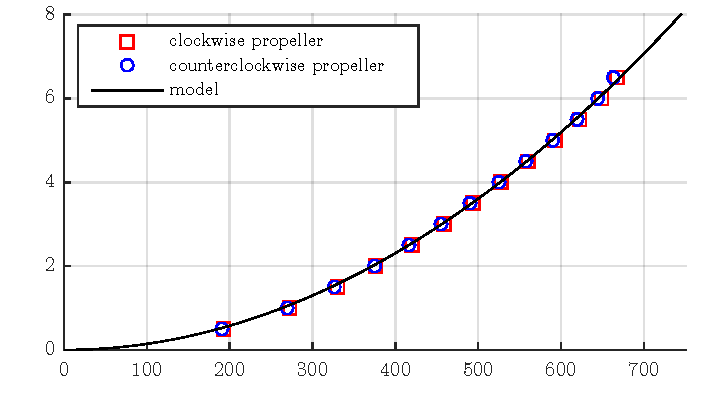
\includegraphics[scale=0.7]{PropVel2Thrust}
%  \caption{Identification of the torque constant $\kappaF$}
%  \label{fig:PropVel2Thrust}
% \end{figure}
% 
% \paragraph*{Identification of the thrust dynamics.}
% For identification of the parameters $\kappaT$, $\BLDCTorqueConstant$ and $\BLDCFriction$ we apply a stair-like input signal for $\BLDCCurr$ (see \autoref{fig:PropIdentMeas}) to the BLDC driver.
% A Savitzky-Golay-filter is applied to the measured propeller velocity $\PropVel$ which also yields an approximation of its derivative $\PropVeld$.
% Finally, knowing the Propeller inertia $\PropInertia$ and the sampled measurements $\PropVel[k]$, $\PropVeld[k]$ and $\BLDCCurr[k]$, we can identify the parameters $\kappaT$, $\BLDCTorqueConstant$ and $\BLDCFriction$ by the method of least squares.
% Overall the propeller drive model parameters are
% \begin{align}
%  \PropInertia &= 2.83 \cdot 10^{-5}\,\tfrac{\unit{N}\,\unit{m}\,\unit{s}^2}{\unit{RAD}},&
%  \kappaF &= 1.44 \cdot 10^{-5} \, \tfrac{\unit{N}\, \unit{s}^2}{\unit{RAD}^2},&
%  \kappaT &= 1.84 \cdot 10^{-7} \, \tfrac{\unit{N}\, \unit{m}\, \unit{s}^2}{\unit{RAD}^2},
% \nonumber\\
% &&
%  \BLDCTorqueConstant &= 1.39 \cdot 10^{-4} \unit{N}\, \unit{m},&
%  \BLDCFriction &= 4.97 \cdot 10^{-3} \unit{N}\, \unit{m}
%  .
% \end{align}
% The simulation result of the propeller model \eqref{eq:PropDriveModelVel} with the identified parameters is also shown in \autoref{fig:PropIdentMeas}.
% 
% Rather than the angular velocity $\PropVel$ we are actually interested in the thrust $\PropForce$ generated by the propeller.
% Elimination of the angular velocity $\PropVel$ from the model equations \eqref{eq:PropDriveModelVel} yields
% \begin{align}\label{eq:PropDriveModelForce}
%  \PropForceTimeConstant(\PropForce\,) \PropForced + \PropForce &= \PropForceInput(\BLDCCurr),
% \end{align}
% where
% \begin{align}
%  \PropForceTimeConstant(\PropForce\,) = \tfrac{\PropInertia \sqrt{\kappaF} }{2\kappaT \sqrt{\PropForce}} = \tfrac{\PropInertia}{2\kappaT \PropVel},
% \quad
%  \PropForceInput(\BLDCCurr) = \tfrac{\kappaF \BLDCTorqueConstant}{\kappaT} \BLDCCurr - \tfrac{\kappaF \BLDCFriction}{\kappaT}
%  .
% \end{align}
% The input characteristic $\PropForceInput(\BLDCCurr)$ is the stationary thrust for a constant input $\BLDCCurr$ and the time characteristic $\PropForceTimeConstant(\PropForce\,)$ corresponds to the time constant for a linear approximation about the working point $\PropForce$. 
% In \autoref{fig:PropIdentRes} the identified characteristics $\PropForceInput(\BLDCCurr)$ and $\PropForceTimeConstant(\PropForce\,)$ are compared to the measurements.
% 
% \paragraph*{Saturation.}
% One can see the beginning of a saturation for the stationary thrust $\PropForceInput$ which becomes stronger for a lower supply voltage (battery) to the power electronics.
% However, since this effect is far away from usual working conditions ($\PropForce \approx 2.5\,\unit{N}$ for quadcopter and $\PropForce \approx 4\,\unit{N}$ for tricopter hover) it is not considered in the model.
% Consequently the least squares identification of the model parameters is also only performed on measurement data for which $\BLDCCurr \leq 600$ to have a good model in the typical working regime.
% 
% \begin{figure}[p]
%  \centering
%  \includegraphics[scale=0.7]{PropIdentMeas.pdf}
%  \caption{Measurements for identification and simulation result}
%  \label{fig:PropIdentMeas}
% \vspace{15mm}
%  \includegraphics[scale=0.7]{PropIdentRes.pdf}
%  \caption{Identified input $\PropForceInput(\BLDCCurr)$ and time characteristic $\PropForceTimeConstant(\PropForce\,)$ of the propeller drive}
%  \label{fig:PropIdentRes}
% \end{figure}
% 
% \paragraph*{Observer.}
% The velocity measurement $\PropVelMeas[]$ is noisy, so it should not be used directly for feedback control.
% On the other hand, Low-pass filtering would lead to undesired delay.
% A solution is the use of an observer which can be regarded as a low-pass filter with a feed forward term that eliminates the delay.
% The implementation is a copy of the forward Euler discretization of the nonlinear model \eqref{eq:PropDriveModelVel} supplemented by a linear feedback of the error to the measurement
% \begin{multline}\label{eq:PropObserver}
%  \PropForceObs[][k] = \kappaF (\PropVelObs[][k])^2, \qquad
%  \tfrac{\PropInertia}{\Ts} (\PropVelObs[][k+1] - \PropVelObs[][k]) + \kappaT (\PropVelObs[][k])^2 = \BLDCTorqueConstant \BLDCCurr[][k] - \BLDCFriction
% \\
%  + l_{\PropVel} \big( \PropVelMeas[][k] - \tfrac{1}{2}(\PropVelObs[][k] + \PropVelObs[][k-1]) \big)
%  .
% \end{multline}
% Note that this leads to second order dynamics for the observer error due to the delay of the measurement.
% However, for reasonable values of the observer gain $l_{\PropVel}$ there is a very fast ``eigenvalue`` that can be neglected and a slower one that can be tuned with the observer gain.
% % closed loop
% % \begin{align}
% %  \PropVelObsErr[][k+1] + \big( \tfrac{2\Ts\kappaT \PropVel[]}{\PropInertia} + \tfrac{\Ts l_{\PropVel}}{2\PropInertia} - 1 \big) \PropVelObsErr[][k] + \tfrac{\Ts l_{\PropVel}}{2\PropInertia} \PropVelObsErr[][k-1] &= \tfrac{\Ts l_{\PropVel}}{\PropInertia} n[k]
% % \end{align}
% 
% \paragraph*{Prefilter.}
% The higher level controllers compute the desired thrust $\PropForceD[][k+1]$ for the next sampling step.
% Since the propeller thrust $\PropForce[]$ has a dynamic of its own \eqref{eq:PropDriveModelForce}, it is not possible to track this signal exactly (without additional information).
% 
% \fixme{
% We consider a combination of a prefilter and a feedback of the error \wrt to the filtered reference $\PropForceDFilt$.
% This approach is sometimes called \fixme{\textit{two degrees of freedom controller}} (\eg \cite{Zeitz:FlatnessSISO}) since it allows independent tuning of the tracking behavior and the closed loop stability.
% }
% 
% The implemented prefilter is the exact discretization of a low-pass filter with the time constant $\TPropForceFilter > \Ts$
% \begin{align}\label{eq:PropPrefilter}
%  \PropForceDFilt[][k+2] = \cPropForceFilter \PropForceDFilt[][k+1] + (1-\cPropForceFilter) \PropForceD[][k+1],
% \qquad
%  \cPropForceFilter = \exp (-\tfrac{\Ts}{\TPropForceFilter})
%  .
% \end{align}
% Note that for the filtered desired thrust $\PropForceDFilt[][k+1]$, we also have the value for the next sampling step $\PropForceDFilt[][k+2]$.
% 
% \paragraph*{Tracking controller.}
% For the tracking error $\PropForceE[]$ we set the desired response as
% \begin{align}\label{eq:ProperrorDyn}
%  \PropForceE[][k+1] = \PropCtrlParam[][k] \, \PropForceE[][k],
% \qquad
%  \PropForceE[][k] = \PropForceDFilt[][k] - \PropForceObs[][k]
%  .
% \end{align}
% Combination with the (forward Euler) discretization of the model \eqref{eq:PropDriveModelForce} yields the corresponding control law
% \begin{multline}\label{eq:PropController}
%  \BLDCCurr[][k+1]
%  = \underbrace{\tfrac{\kappaT}{\kappaF\BLDCTorqueConstant}\big( \tfrac{\PropInertia}{2 \kappaT \Ts \PropVelObs[][k+1]} \big(\PropForceDFilt[][k+2] - \PropForceDFilt[][k+1]\big) + \PropForceDFilt[][k+1] \big) + \tfrac{\BLDCFriction}{\BLDCTorqueConstant}}_{\text{feed-forward}}
% \\[-1.5ex]
%  + \overbrace{\underbrace{\tfrac{\kappaT}{\kappaF\BLDCTorqueConstant}\big( \tfrac{\PropInertia (1 - \PropCtrlParam[][k+1])}{2 \kappaT \Ts \PropVelObs[][k+1]} - 1 \big)}_{K_\textsf{FC}[k+1]}\PropForceE[][k+1]}^{\text{feedback}}
% \end{multline}
% 
% The closed loop parameter $\PropCtrlParam[][k]$ introduced in \eqref{eq:ProperrorDyn} is chosen as an affine function of the current (observed) angular velocity
% \begin{align}\label{eq:PropCtrlParam}
%  \PropCtrlParam[][k] = \PropCtrlParam[0] + \PropCtrlParam[1] \PropVelObs[][k]
%  .
% \end{align}
% Choosing $\PropCtrlParam[1]=0$ would lead to linear error dynamics, but would result in a high feedback gain $K_\textsf{FC}$ at low velocity $\PropVel$.
% On the other hand choosing $\PropCtrlParam[0]=1$ would lead to a constant feedback gain $K_\textsf{FC}$ which is too strong at high and too weak at low velocities.
% With \eqref{eq:PropCtrlParam} one can find a practical balance between these extreme cases.
% 
% \paragraph*{Tuning and validation.}
% The following parameters are used for the propeller control
% \begin{align}
%  l_{\PropVel} &= 7 \cdot 10^{-4}\, \tfrac{\unit{kg}\,\unit{m}^2}{\unit{s}},&
%  \TPropForceFilter &= 4 \Ts = 0.02\,\unit{s},&
%  \PropCtrlParam[0] &= 0.95,&
%  \PropCtrlParam[1] &= -8.40 \cdot 10^{-5} \unit{s}
%  .
% \end{align}
%  \autoref{fig:PropCtrlRes}.
% 
% \begin{figure}[h!]
%  \centering
%  \includegraphics[scale=0.7]{PropTimeCharacteristics.pdf}
%  \caption{Time characteristic of the propeller thrust control}
%  \label{fig:PropTimeCharacteristics}
% \end{figure}
% 
% 
% 
% \subsection{Servo model}
% The tiling mechanisms of the Tricopter are driven by hobbyist servo motors.
% Each is interfaced by a pulse width modulated signal corresponding to the desired angle $\aServoR$.
% 
% We consider the second order model whose parameters have been identified with a dedicated experiment
% \begin{align}
%  \aServodd + 2\zetaServo \wServo \aServod + \wServo^2 \aServo = \wServo^2 \aServoR,
% \qquad
%   \wServo = 39\,\unit{s}^{-1}, \ \zetaServo = 0.93
% \end{align}
% 
% Discrete simulator for the servo angle using the forward Euler approximation
% \begin{subequations}
% \begin{align}
%  \aServoObs[][k+1] &= \aServoObs[][k] + \Ts \aServoObsd[][k]
% \\
%  \aServoObsd[][k+1] &= \aServoObsd[][k] + \Ts( \wServo^2 (\aServoR[][k] - \aServoObs[][k]) - 2\zetaServo \wServo \aServoObsd[][k])
%  .
% \end{align}
% \end{subequations}
% 
% See \autoref{fig:ServoObsRes}.
% 
% \begin{figure}[p]
%  \centering
%  \includegraphics[scale=0.65]{PropCtrlRes/PropCtrlRes.pdf}
% % \vspace{-2mm}
%  \caption{Thrust control result}
%  \label{fig:PropCtrlRes}
% \vspace{3ex}
%  \includegraphics[scale=0.65]{ServoSimRes/ServoSimRes.pdf}
% % \vspace{-2mm}
%  \caption{Comparison of measured and simulated servo angle}
%  \label{fig:ServoObsRes}
% \end{figure}